\documentclass[12pt]{exam}		%Doc : https://mirrors.ircam.fr/pub/CTAN/macros/latex/contrib/exam/examdoc.pdf
\printanswers					%Comment this line to hide the answers 
\usepackage[utf8]{inputenc}
\usepackage[T1]{fontenc}
\usepackage[french]{babel}      %Originally for french document, change to english or relevant language

\usepackage{amsmath,amssymb}
\usepackage{multicol}
\usepackage[dvipsnames]{xcolor}
\usepackage[shortlabels]{enumitem}
\usepackage{tikz}
	\usetikzlibrary{fadings}
	\usetikzlibrary{calc}
	
\usepackage{tkz-tab}
\usepackage{pgfplots}

%Format Header and footer
\pagestyle{headandfoot}
\header{\footnotesize Class\\Id number}{\Large\textbf{Name}}
\headrule
\footrule
\setlength{\columnsep}{0.25cm}
%\setlength{\columnseprule}{1pt}
\footer{}{Page \thepage}{}
%\extrafootheight{-2cm}

% Change section command behaviour
\usepackage{titlesec}
\titleformat{\section}[frame]{\Huge\bfseries\filright}{}{2mm}{\centering Chemistry 107 :\ }

% Add a watermark if answers are shown
%\ifprintanswers
%\usepackage{draftwatermark}
%\SetWatermarkColor{red!30}
%\SetWatermarkScale{5}
%\SetWatermarkText{Solution}     %Watermark text
%\fi

%Format the name of each exercise
\qformat{\textbf{Exercice \thequestion~:}\hfill}
\extrawidth{1.5cm}

\begin{document}
\section{Exam 1B}

\noindent The 100 pts exam consists of 9 questions and students have 1.5 hours to complete the exam.
Answers must be written in the box provided or else no credit is provided. Use the empty
space provided to do your work. A periodic table is provided at the end. Fill in your name along with your
student ID number.
\\

\noindent\textbf{Problem 1: Sig Figs} Solve the following equations with the appropriate number of
significant figures (10 pts)
\\
\begin{enumerate}[(a)]
\item \begin{equation*}
  5.192\times 10^2 - 1.024 \times 10 =
  \end{equation*}
  \vspace{0.1in}
\item[]\tikz[baseline=1ex]\draw (0,0) rectangle (17cm,5ex);
\item \begin{equation*}
  \frac{67.12 +52.013}{45.1} =
  \end{equation*}
  \vspace{0.1in}
\item[]\tikz[baseline=1ex]\draw (0,0) rectangle (17cm,5ex);
\item \begin{equation*}
  \frac{1.25\times 10^{-3} + 8.\times 10^{-4}}{7.51}
  \end{equation*}
  \vspace{0.1in}
\item[]\tikz[baseline=1ex]\draw (0,0) rectangle (17cm,5ex);
\item \begin{equation*}
  \frac{145\text{g}}{80.17\text{mL} - 15.32\text{mL}} =
  \end{equation*}
  \vspace{0.1in}
\item[]\tikz[baseline=1ex]\draw (0,0) rectangle (17cm,5ex);
\item \begin{equation*}
  (3.198 \times 10^4)(9.18 \times 10^{-2}) =
  \end{equation*}
  \vspace{0.1in}
\item[]\tikz[baseline=1ex]\draw (0,0) rectangle (17cm,5ex);
\end{enumerate}

\newpage

\noindent\textbf{Problem 2: Unit Conversion} Convert the following units. (12 pts)
\\
\begin{enumerate}[(a)]
\item 58.58 ms to Ms %
\item[]\tikz[baseline=1ex]\draw (0,0) rectangle (17cm,5ex);
\item 129.1 mm$^2$ to km$^2$ %
\item[]\tikz[baseline=1ex]\draw (0,0) rectangle (17cm,5ex);
\item 8.16 dag/L to dg/mL %Cloric acid
\item[]\tikz[baseline=1ex]\draw (0,0) rectangle (17cm,5ex);
\item 1 ML to m$^3$ %Ammonium Sulfate
\item[]\tikz[baseline=1ex]\draw (0,0) rectangle (17cm,5ex);
\item 43.007 nHz to kHz %H2CO3
\item[]\tikz[baseline=1ex]\draw (0,0) rectangle (17cm,5ex);
\item 325.48 Kelvin to $^\circ$C %NaHCO3
\item[]\tikz[baseline=1ex]\draw (0,0) rectangle (17cm,5ex);
\end{enumerate}
\vspace{0.3in}

\noindent\textbf{Problem 3: Empirical and Molecular Formulas} Caffeine, a
stimulant in coffee and tea, has a molar mass of 194.19 g/mol and a mass percentage
composition of $49.48\%$ C, $5.19\%$ H, $28.85\%$ N, and $16.48\%$ O. (8 pts)
\\
\begin{enumerate}[(a)]
\item Determine the empirical formula  %H2CO3
  \vspace{1in}
\item[]\tikz[baseline=1ex]\draw (0,0) rectangle (17cm,5ex);
\item What is the molecular formula of caffeine?  %NaHCO3
  \vspace{1in}
\item[]\tikz[baseline=1ex]\draw (0,0) rectangle (17cm,5ex);
\end{enumerate}

\newpage

\noindent\textbf{Problem 4: Molarity} Barium Chloride (BaCl$_2$) is a water-soluble inorganic
compound that is toxic and shines yellow-and green under a flame. It has wide applications
in the laboratory and in industry such as steel manufracture. Report all results
to 3 significant figures. (12 pts)
\\
\begin{enumerate}[(a)]
\item Determine the mass percent of each element in BaCl$_2$.
  \vspace{2in}
\item[]\tikz[baseline=1ex]\draw (0,0) rectangle (17cm,5ex);
\item A scientist attempts to prepare 1.50L of 1.75M BaCl$_2$. How many grams of
  BaCl$_2$ is needed?
  \vspace{2in}
\item[]\tikz[baseline=1ex]\draw (0,0) rectangle (17cm,5ex);
\item Suppose the solution in part b) needs to be diluted to make
  3.75L of 0.5M BaCl$_2$, how much volume in L is needed from 1.75M BaCl$_2$?
  \vspace{2in}
\item[]\tikz[baseline=1ex]\draw (0,0) rectangle (17cm,5ex);
\end{enumerate}

\newpage

\noindent\textbf{Problem 5: Short Answer} Scientists attempt to understand chemical
phenomena and solve problems using the scientific method. What is the scientific
method? Describe an everyday example in which you use the scientific method. (8 pts)
\vspace{0.3in}

\tikz[baseline=1ex]\draw (0,0) rectangle (17.5cm,47ex);

\vspace{0.3in}

\noindent\textbf{Problem 6: Nomenclature} Provide either the molecular formula or
compound name for the following. (12 pts)
\\
\begin{enumerate}[(a)]
\item Vanadium(V) acetate %V(C2H3O2)5
\item[]\tikz[baseline=1ex]\draw (0,0) rectangle (17cm,5ex);
\item Sr(C$_2$H$_3$O$_2$) %Strontium Acetate
\item[]\tikz[baseline=1ex]\draw (0,0) rectangle (17cm,5ex);
\item HClO$_3$ %Cloric acid
\item[]\tikz[baseline=1ex]\draw (0,0) rectangle (17cm,5ex);
\item (NH$_4$)$_2$SO$_4$ %Ammonium Sulfate
\item[]\tikz[baseline=1ex]\draw (0,0) rectangle (17cm,5ex);
\item Carbonic acid %H2CO3
\item[]\tikz[baseline=1ex]\draw (0,0) rectangle (17cm,5ex);
\item Sodium bicarbonate %NaHCO3
\item[]\tikz[baseline=1ex]\draw (0,0) rectangle (17cm,5ex);
\end{enumerate}

\newpage

\noindent\textbf{Problem 7: Relative Atomic Mass} Boron has only two naturally occurring
isotopes (Boron-10 and Boron-11). The mass of Boron-10 is 10.01294 amu and the mass of
Boron-11 is 11.00931 amu. Report to 3 significant figures. (10 pts)
\\
\begin{enumerate}[(a)]
\item Based on the periodic table, which boron isotope has the greater relative
  abundance? Explain using words and/or formulas.
\item[]\tikz[baseline=1ex]\draw (0,0) rectangle (17cm,26ex);
\item Calculate the relative abundance of each isotope. \textit{Hint:} There are two
  equations required. Set up a system of equations using the relative atomic mass
  formula and the relative abundance.
  \vspace{1.75in}
\item[]\tikz[baseline=1ex]\draw (0,0) rectangle (17cm,5ex);
\end{enumerate}
\vspace{0.3in}
\noindent\textbf{Problem 8: Atoms and Ions} Complete the table with the symbol,
atomic number $Z$, atomic mass $A$, number of protons ($p^+$), number of electrons
$e^-$, number of neutrons $n$, and charge. (8 pts)
\\
\begin{table}[hbpt]
  \centering
  \Large
  \begin{tabular}{c|cccccc}
    Symbol & $Z$ & $A$ & $p^+$ & $e^-$ & $n$ & Charge \\
    \hline\hline
    Si      & 14 & & 14 & 14 & 15 & \\
    S$^{2-}$ & & 32 & & & & \\
    & 29 & & & & 13 & 2+ \\
    & 15 & & & 18 & 16 & \\
    Fe$^{2+}$ & & 56 & & & \\
    \hline
  \end{tabular}
\end{table}

\newpage

\noindent\textbf{Problem 9: True/False } Determine whether the statement is true or false. (20 pts)
\\
\begin{enumerate}[(a)]
\item An element is a pure substance that contains only one type of atom. %True
\item[]\tikz[baseline=1ex]\draw (0,0) rectangle (17cm,5ex);
\item Atoms are indivisible and indestructible. %False
\item[]\tikz[baseline=1ex]\draw (0,0) rectangle (17cm,5ex);
\item The atomic number of a substance is the number of neutrons that an
  element has. %False
\item[]\tikz[baseline=1ex]\draw (0,0) rectangle (17cm,5ex);
\item The mass of an atom is the sum of the masses of neutrons, protons, and
  electrons. %True
\item[]\tikz[baseline=1ex]\draw (0,0) rectangle (17cm,5ex);
\item When a chemical change occurs, matter keeps the same chemical
  properties. %False
\item[]\tikz[baseline=1ex]\draw (0,0) rectangle (17cm,5ex);
\item The total moles of reactants must equal the total moles of
  products. %\False
\item[]\tikz[baseline=1ex]\draw (0,0) rectangle (17cm,5ex);
\item Matter and energy are neither created nor destroyed. %True
\item[]\tikz[baseline=1ex]\draw (0,0) rectangle (17cm,5ex);
\item All Br{\o}nsted acids are Lewis acids. %True
\item[]\tikz[baseline=1ex]\draw (0,0) rectangle (17cm,5ex);
\item Given a solution at concentration $M$, when the volume of the solution
  is increased by 2 times, then concentration is halved. %True
\item[]\tikz[baseline=1ex]\draw (0,0) rectangle (17cm,5ex);
\item Creating metal alloys such as steel and bronze is considered a physical change. %True
\item[]\tikz[baseline=1ex]\draw (0,0) rectangle (17cm,5ex);        
\end{enumerate}

\newpage

\appendix

\begin{center}
  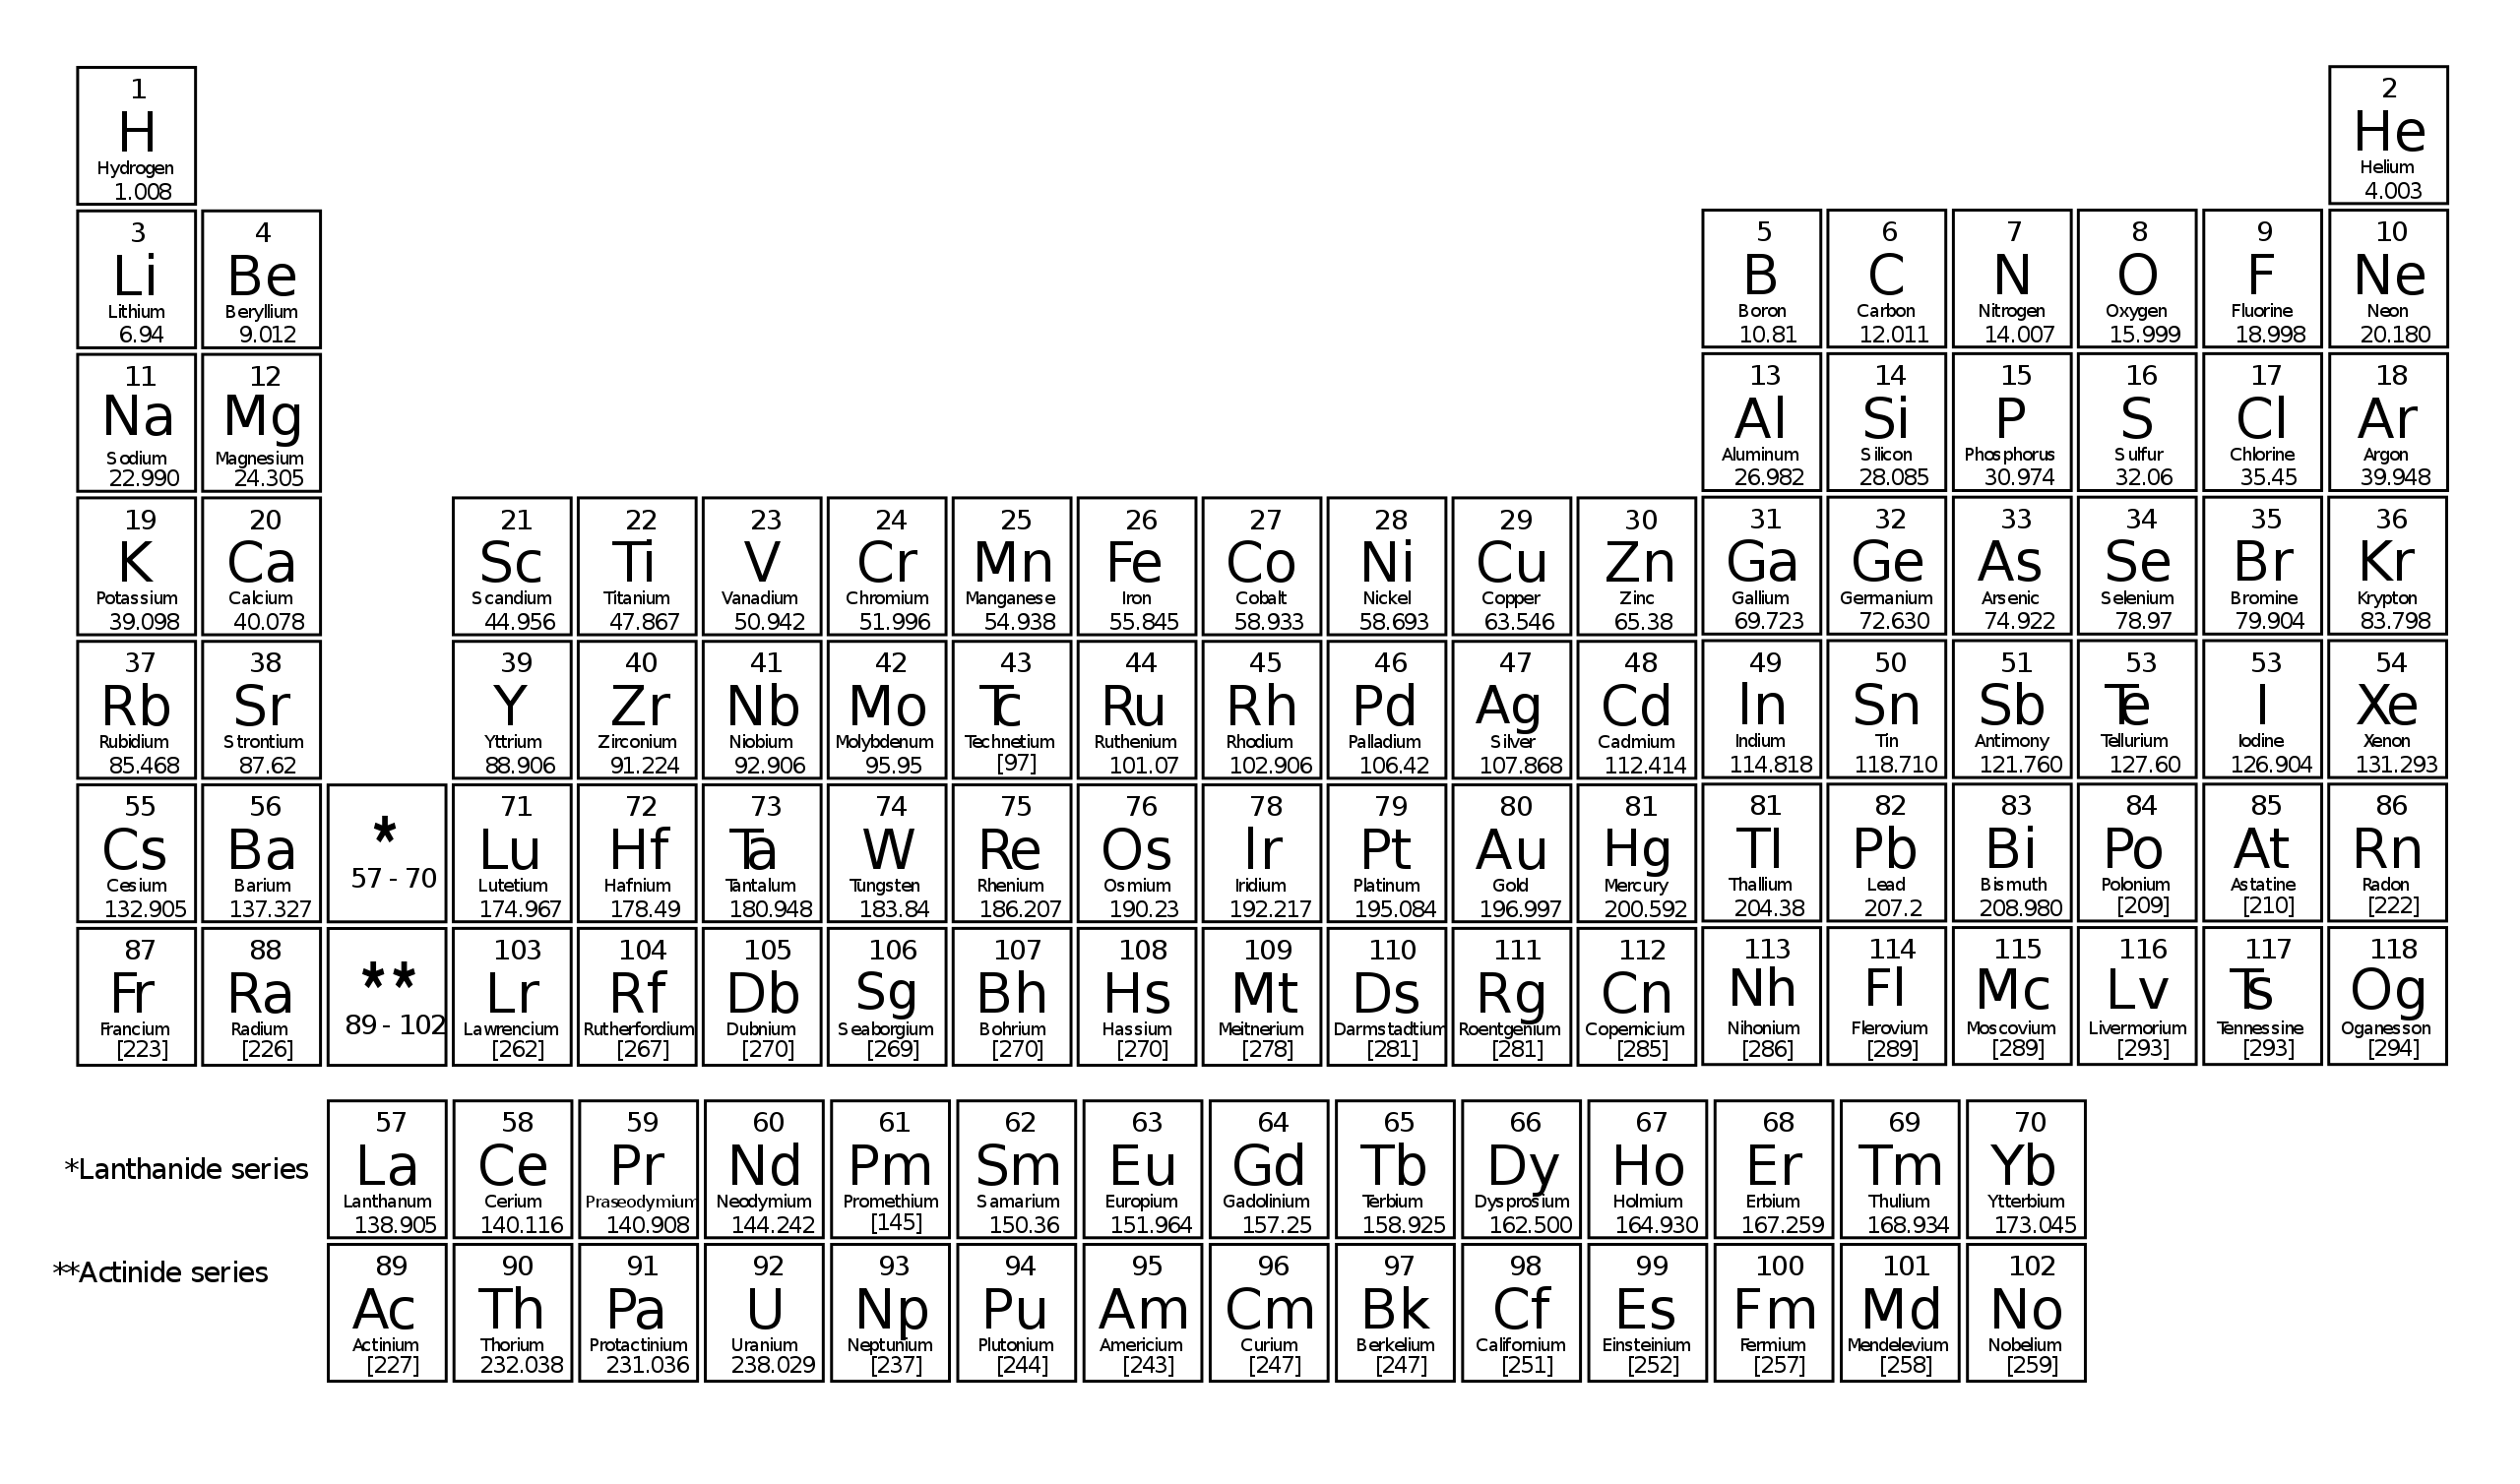
\includegraphics[scale=0.26,angle=90]{periodic_table}
\end{center}

\end{document}
